%-*- coding=utf-8 -*-
\documentclass[UTF8]{ctexart}
\usepackage{geometry}
\CTEXsetup[format={\Huge\bfseries}]{section}
\CTEXsetup[format={\LARGE\bfseries}]{subsection}
%\usepackage{titlesec}
\geometry{left=3.18cm,right=3.18cm,top=2.54cm,bottom=2.54cm}
\usepackage{graphicx}
\pagestyle{plain}	
% \usepackage{booktabs}
% \usepackage{subfigure}
\usepackage{setspace}
\usepackage{float}
\begin{document}
	\begin{center}
		\quad \\
		\quad \\
		\heiti \fontsize{45}{17} 高级网络编程
		\vskip 2.0cm
		\heiti \fontsize{39}{17} 实验报告	
	\end{center}
	\vskip 3.5cm
	\begin{quotation}
		\par\setlength\parindent{8.5em}
		\quad 
		\heiti 
		
		实验名称:基本名字与地址转换
		
		实验日期:2020年5月22日
	
		学生姓名:黄文政
		
		学\hspace{0.72cm}号:71Y17111
		
		\vskip 2cm
		\centering
	\end{quotation}
	
\newpage
\songti \fontsize{13}{13}
\large
\section*{一、实验目的}

1. 掌握应用程序进行主机名和IP地址间转换的过程。

2. 掌握各种转换函数的使用方法。


\section*{二、实验环境}
windows 10

\section*{三、实验内容}
\subsection*{\textbf{1. 应用程序进行主机名和IP地址间转换的过程}}
\subsection*{1.1 主要过程}

当一个应用进程发出解析域名的请求时,会发生下列活动:

1. 解析器查找本机设定的本地DNS服务器的IP地址

2. 以上述IP地址为目标发送UDP包,请求进行域名解析

3. 若本地DNS服务器无法解析,则继续往上层DNS服务器发送请求,直到解析成功

\subsection*{\textbf{2. 各种转换函数的使用方法}}
\subsection*{2.1 设计思路}

使用windows socket API,调用下列函数并观察结果:

gethostname(), gethostbyname(), gethostbyaddr(), getservbyname(), getservbyport()

\subsection*{2.2 运行结果}

\begin{figure}[H]
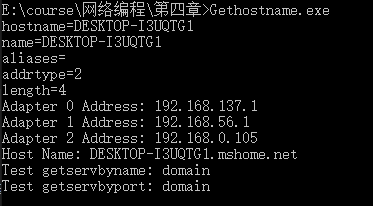
\includegraphics[width=\textwidth]{pic/DNS.PNG}
\caption{名字解析程序运行结果}
\end{figure}

结果显示了gethostbyname()函数返回的实验机器主机名(hostname)、协议族(2,即AF\_INET)、地址长度
(length=4)。实验机器的网络适配器有三个,并有不同的IP地址。gethostbyaddr()函数获取的主机名为
"DESKTOP-I3UQTG1.mshome.net",与gethostname()函数的结果不同。getservbyname()和getservbyport()
函数则分别根据传入的名字或端口获取对应服务的详细信息,如此处传入的服务名字为"domain",端口为53,则获取
到了DNS服务的信息。

\section*{四、实验总结}

本次实验主要调通了Gethostname.cpp程序,并了解了各种转换函数的使用方法。需要注意编译时要链接
ws2\_32.dll(ws2\_32.dll是Windows\ Sockets应用程序接口, 用于支持Internet和网络应用程序)。由于实验
机器的domain服务没有别名,故将打印s\_aliases改成打印s\_name。

\end{document}